\documentclass[12pt]{beamer}
% ---------- doc 1 format: 12pt, lmodern serif, pale-blue title band, triangle bullets ----------
\usepackage{lmodern}
\usefonttheme{serif}
\usepackage{amsmath,amssymb}
\usepackage{booktabs}
\usepackage{pgfplots}
\pgfplotsset{compat=1.18}

\definecolor{lectureblue}{RGB}{0,70,150}
\definecolor{paleblue}{RGB}{221,233,248}
\definecolor{examplegreen}{RGB}{0,120,60}

\setbeamertemplate{navigation symbols}{}
\setbeamertemplate{itemize item}[triangle]
\setbeamertemplate{itemize subitem}[triangle]
\setbeamercolor{itemize item}{fg=lectureblue}
\setbeamercolor{itemize subitem}{fg=lectureblue}
\setbeamercolor{frametitle}{bg=paleblue,fg=black}
\setbeamerfont{frametitle}{size=\large,series=\bfseries}
\setbeamertemplate{frametitle}{%
  \nointerlineskip
  \begin{beamercolorbox}[wd=\paperwidth,ht=2.6ex,dp=1.1ex,leftskip=0.45cm]{frametitle}%
    \usebeamerfont{frametitle}\insertframetitle
  \end{beamercolorbox}}
\setbeamercolor{title}{fg=lectureblue}
\setbeamertemplate{footline}{\hfill\scriptsize\insertframenumber\hspace*{0.3cm}\vspace*{0.15cm}}

\newcommand{\keyterm}[1]{\textcolor{examplegreen}{\textbf{#1}}}
\newcommand{\fitO}{}
\newcommand{\exlists}{\setlength{\itemsep}{0pt}}
\newcommand{\ind}[1]{\hspace*{#1}}
\newcommand{\Xbar}{\overline{X}}

\title{Section 5.4}
\subtitle{The Distribution of the Sample Mean}
\date{}

\begin{document}

% ======================================================================
\begin{frame}
\titlepage
\end{frame}

% ======================================================================
\begin{frame}[t]{Recall: Random Samples}
\begin{itemize}
\item A \keyterm{random sample} $X_1,\dots,X_n$ satisfies:
  \begin{itemize}
  \item the $X_i$'s are independent;
  \item every $X_i$ has the same distribution.
  \end{itemize}
\item[]
\item The \keyterm{sample mean} is the statistic
\[
\textcolor{blue}{\Xbar=\frac{1}{n}\sum_{i=1}^{n}X_i}
\]
\item $\Xbar$ is a random variable, so it has a distribution: the
  \keyterm{sampling distribution} of $\Xbar$.
\item[]
\item Today: the mean, variance and shape of this distribution.
\end{itemize}
\end{frame}

% ======================================================================
\begin{frame}[t]{Mean and Variance of $\Xbar$}
\begin{itemize}
\item Let $X_1,\dots,X_n$ be a random sample from a distribution with
  mean $\mu$ and standard deviation $\sigma$. Then
\[
\textcolor{blue}{E(\Xbar)=\textcolor{magenta}{\mu_{\Xbar}}=\mu}
\qquad
\textcolor{blue}{V(\Xbar)=\textcolor{magenta}{\sigma^2_{\Xbar}}=\frac{\sigma^2}{n}}
\qquad
\textcolor{blue}{\textcolor{magenta}{\sigma_{\Xbar}}=\frac{\sigma}{\sqrt{n}}}
\]
\item For the \keyterm{sample total} $T_0=X_1+\cdots+X_n$:
\[
\textcolor{red}{E(T_0)=n\mu}
\qquad
\textcolor{red}{V(T_0)=n\sigma^2}
\qquad
\textcolor{red}{\sigma_{T_0}=\sqrt{n}\,\sigma}
\]
\item $\Xbar$ is centered at the population mean $\mu$.
\item The spread of $\Xbar$ shrinks as $n$ grows.
\item $\sigma_{\Xbar}=\sigma/\sqrt{n}$ is called the \keyterm{standard error} of the mean.
\end{itemize}
\end{frame}

% ======================================================================
%% answers: a) E(Xbar)=500, V(Xbar)=100/25=4, sigma_Xbar=2
%%          b) E(T0)=25(500)=12500, V(T0)=25(100)=2500, sigma_T0=50
%%          c) sigma_Xbar=10/sqrt(100)=1 (halved)
\begin{frame}[t]{}\fitO\exlists
\textcolor{blue}{\textbf{Example 1:}}\,\ The fill weight of a cereal box has
mean $\mu=500$ g and standard deviation $\sigma=10$ g. A random sample of
$n=25$ boxes is selected.
\begin{itemize}
\item[a)] Find $E(\Xbar)$, $V(\Xbar)$ and $\sigma_{\Xbar}$.\\[0.2cm]
\end{itemize}
\end{frame}

\begin{frame}[t]{}\fitO\exlists
\begin{itemize}
\item[b)] Find $E(T_0)$, $V(T_0)$ and $\sigma_{T_0}$, where $T_0$ is the total weight of the 25 boxes.\\[3.4cm]
\item[c)] What is $\sigma_{\Xbar}$ if the sample size is increased to $n=100$?\\[0.2cm]
\end{itemize}
\end{frame}

% ======================================================================
\begin{frame}[t]{The Case of a Normal Population}
\begin{itemize}
\item Let $X_1,\dots,X_n$ be a random sample from a normal distribution,
  $X_i\sim N(\mu,\sigma^2)$. Then, for \textbf{every} $n$,
\[
\textcolor{blue}{\Xbar\sim N\!\left(\mu,\ \frac{\sigma^2}{n}\right)}
\qquad
\textcolor{blue}{T_0\sim N\!\left(n\mu,\ n\sigma^2\right)}
\]
\item Probabilities are found by standardizing:
\[
\textcolor{red}{Z=\frac{\Xbar-\mu}{\sigma/\sqrt{n}}\sim N(0,1)}
\qquad
\textcolor{red}{Z=\frac{T_0-n\mu}{\sqrt{n}\,\sigma}\sim N(0,1)}
\]
\item This result is exact: no large-sample condition is needed.
\end{itemize}
\end{frame}

% ======================================================================
%% answers: sigma_Xbar = 2/4 = 0.5
%%   a) P(Xbar<=12.5)=Phi(1.00)=0.8413
%%   b) P(11.5<=Xbar<=12.5)=Phi(1)-Phi(-1)=0.6826
%%   c) T0~N(192, 64), sd 8: P(T0>200)=1-Phi(1.00)=0.1587
\begin{frame}[t]{}\fitO\exlists
\textcolor{blue}{\textbf{Example 2:}}\,\ The time (in minutes) a worker needs to
assemble a part is normally distributed with mean 12 and standard deviation 2.
A random sample of $n=16$ workers is observed.
\begin{itemize}
\item[a)] Find $P(\Xbar\le 12.5)$.\\[0.2cm]
\end{itemize}
\end{frame}

\begin{frame}[t]{}\fitO\exlists
\begin{itemize}
\item[b)] Find $P(11.5\le \Xbar\le 12.5)$.\\[3.4cm]
\item[c)] Find the probability that the total time of the 16 workers is more than 200 minutes.\\[0.2cm]
\end{itemize}
\end{frame}

% ======================================================================
\begin{frame}[t]{The Central Limit Theorem}
\begin{itemize}
\item Let $X_1,\dots,X_n$ be a random sample from \textbf{any} distribution with
  mean $\mu$ and variance $\sigma^2$. If $n$ is sufficiently large, then
\[
\textcolor{blue}{\Xbar\ \text{ is approximately }\ N\!\left(\mu,\ \frac{\sigma^2}{n}\right)}
\]
\[
\textcolor{blue}{T_0\ \text{ is approximately }\ N\!\left(n\mu,\ n\sigma^2\right)}
\]
\item The larger $n$ is, the better the approximation.
\item Rule of thumb: the \keyterm{Central Limit Theorem} (CLT) may be used if $n>30$.
\item If the population is already normal, $\Xbar$ is exactly normal for every $n$.
\end{itemize}
\end{frame}

% ======================================================================
\begin{frame}[t]{The CLT: An Illustration}
\begin{itemize}
\item Population: exponential with $\mu=1$ (strongly skewed).
\item The pdf of $\Xbar$ for $n=1,\ 5,\ 20$:
\end{itemize}
\vspace{-0.2cm}
\begin{center}
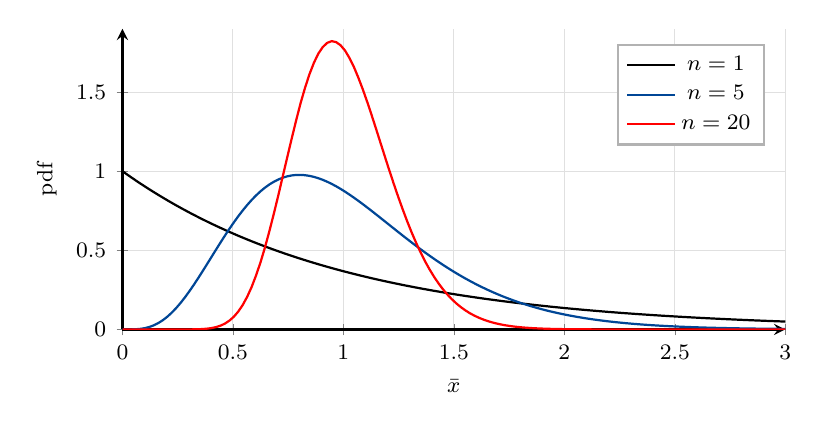
\begin{tikzpicture}
\begin{axis}[
  width=10cm, height=5.4cm,
  xmin=0, xmax=3, ymin=0, ymax=1.9,
  axis lines=left, grid=both, grid style={black!12},
  xlabel={$\bar{x}$}, ylabel={pdf},
  tick label style={font=\footnotesize}, label style={font=\footnotesize},
  legend style={font=\footnotesize, draw=black!30, at={(0.97,0.95)}, anchor=north east},
  samples=150, domain=0.001:3, thick]
\addplot[black] {exp(-x)};
\addplot[lectureblue] {3125/24*x^4*exp(-5*x)};
\addplot[red] {exp(20.5747613 + 19*ln(x) - 20*x)};
\legend{$n=1$, $n=5$, $n=20$}
\end{axis}
\end{tikzpicture}
\end{center}
\vspace{-0.2cm}
\begin{itemize}
\item As $n$ grows, the pdf of $\Xbar$ gets narrower and more bell-shaped around $\mu=1$.
\end{itemize}
\end{frame}

% ======================================================================
%% answers: sigma_Xbar = 3/sqrt(36) = 0.5
%%   a) P(Xbar>4.5) ~ 1-Phi(1.00)=0.1587
%%   b) T0 ~ N(144, 324), sd 18: P(T0<=162) ~ Phi(1.00)=0.8413
%%   c) n=36>30, so the CLT applies even though the call times are skewed
\begin{frame}[t]{}\fitO\exlists
\textcolor{blue}{\textbf{Example 3:}}\,\ The length of a customer service call has
mean 4 minutes and standard deviation 3 minutes. The distribution is skewed to the right.
A random sample of $n=36$ calls is observed.
\begin{itemize}
\item[a)] Find the approximate probability that the sample mean call length is more than 4.5 minutes.\\[0.2cm]
\end{itemize}
\end{frame}

\begin{frame}[t]{}\fitO\exlists
\begin{itemize}
\item[b)] Find the approximate probability that the total length of the 36 calls is at most 162 minutes.\\[3.4cm]
\item[c)] Why can we use the normal distribution here, even though call lengths are not normal?\\[0.2cm]
\end{itemize}
\end{frame}

% ======================================================================
%% answers: mu = 0(.5)+1(.3)+2(.2) = 0.7; E(X^2)=0.3+0.8=1.1; sigma^2=1.1-0.49=0.61
%%   sigma_Xbar = sqrt(0.61/100) = 0.0781
%%   P(Xbar<=0.8) ~ Phi((0.8-0.7)/0.0781) = Phi(1.28) = 0.8997
\begin{frame}[t]{}\fitO\exlists
\textcolor{blue}{\textbf{Example 4:}}\,\ The number of flaws $X$ on a sheet of glass has pmf
\begin{center}
\renewcommand{\arraystretch}{1.3}
\begin{tabular}{c|ccc}
$x$    & 0   & 1   & 2   \\ \hline
$p(x)$ & 0.5 & 0.3 & 0.2 \\
\end{tabular}
\end{center}
A random sample of $n=100$ sheets is inspected.
\begin{itemize}
\item[a)] Find $\mu$ and $\sigma^2$.\\[0.2cm]
\end{itemize}
\end{frame}

\begin{frame}[t]{}\fitO\exlists
\begin{itemize}
\item[b)] Find the approximate probability that the sample mean number of flaws is at most 0.8.\\[0.2cm]
\end{itemize}
\end{frame}

% ======================================================================
\begin{frame}[t]{Other Applications of the CLT}
\begin{itemize}
\item Let $X\sim \text{Bin}(n,p)$. Then $X=X_1+\cdots+X_n$, where
\[
X_i=\begin{cases}1 & \text{if trial } i \text{ is a success}\\ 0 & \text{if trial } i \text{ is a failure}\end{cases}
\]
  so $X$ is a sample total $T_0$, with $\mu=p$ and $\sigma^2=p(1-p)$.
\item By the CLT, for large $n$:
\[
\textcolor{blue}{X\ \text{ is approximately }\ N\big(np,\ np(1-p)\big)}
\]
\item The sample proportion $\hat{p}=X/n$ is a sample mean, so it is approximately
  $N\big(p,\ p(1-p)/n\big)$.
\item Rule of thumb: use this if $np\ge 10$ and $n(1-p)\ge 10$.
\end{itemize}
\end{frame}

% ======================================================================
\begin{frame}[t]{Summary}
\begin{center}
\renewcommand{\arraystretch}{1.4}
\begin{tabular}{lll}
\toprule
Population & Sample size & Distribution of $\Xbar$ \\
\midrule
any        & any $n$     & $E(\Xbar)=\mu,\ \ V(\Xbar)=\sigma^2/n$ \\
normal     & any $n$     & exactly $N(\mu,\sigma^2/n)$ \\
not normal & $n>30$      & approximately $N(\mu,\sigma^2/n)$ (CLT) \\
\bottomrule
\end{tabular}
\end{center}
\vspace{0.3cm}
\begin{itemize}
\item To find probabilities, standardize: $Z=\dfrac{\Xbar-\mu}{\sigma/\sqrt{n}}$.
\item For the total, use $T_0$ with mean $n\mu$ and standard deviation $\sqrt{n}\,\sigma$.
\end{itemize}
\end{frame}

\end{document}
